% !TeX root = relatorio.tex
\documentclass[12pt,a4paper]{article}

\usepackage[T1]{fontenc}
\usepackage[utf8]{inputenc}
\usepackage[brazilian]{babel}
\usepackage{lmodern}
\usepackage[a4paper,margin=2.5cm]{geometry}
\usepackage{amsmath}
\usepackage{amssymb}
\usepackage{graphicx}
\usepackage{float}
\usepackage{booktabs}
\usepackage{hyperref}
\usepackage{xcolor}

\hypersetup{
  colorlinks=true,
  linkcolor=blue,
  urlcolor=blue,
  pdftitle={Relatorio do Trabalho 1},
  pdfauthor={Gustavo Shoiti Sonoda}
}
\urlstyle{tt}

\renewcommand{\contentsname}{Sumário}
\setlength{\parindent}{0pt}
\setlength{\parskip}{0.7em}
\linespread{1.05}

\newcommand{\arquivo}[1]{\nolinkurl{#1}}
\newcommand{\campo}[2]{\textbf{#1.} #2\par}
\newcommand{\figdir}[1]{figuras/exercicio_#1}
\newcommand{\exerciciosubsection}[2]{\subsection{Exercício #1 -- #2}}

\begin{document}
\hypersetup{pageanchor=false}
\pagenumbering{gobble}

\begin{titlepage}
  \centering

  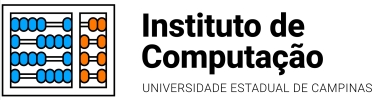
\includegraphics[width=0.24\textwidth]{figuras/logo_ic.png}\par
  \vspace{0.8cm}
  {\large Universidade Estadual de Campinas\par}
  {\large Instituto de Computação\par}

  \vspace{1.5cm}

  {\Large \textbf{Relatório de Implementação do Trabalho 1}\par}
  \vspace{0.5cm}
  {\large Introdução ao Processamento Digital de Imagens (MC920/MO443)\par}
  \vspace{1.2cm}

  {\large Relatório de implementação desenvolvido para a disciplina\\
    Introdução ao Processamento Digital de Imagens.\par}

  \vspace{1.5cm}

  \begin{flushleft}
    \textbf{Professor:} Hélio Pedrini\\
    \textbf{Aluno:} Gustavo Shoiti Sonoda\\
    \textbf{RA:} 217579\\
  \end{flushleft}

  \vfill

  Campinas -- São Paulo\\
  \today
\end{titlepage}

\tableofcontents
\newpage
\hypersetup{pageanchor=true}
\pagenumbering{arabic}

\section{Introdução}

O Trabalho 1 da disciplina MC920/MO443 propõe treze exercícios introdutórios de processamento digital de imagens, cobrindo transformações geométricas, operações pontuais, manipulação de imagens RGB, quantização, decomposição em planos de bits e filtragem espacial. O enunciado pede implementações sem recorrer às funções prontas específicas das bibliotecas quando isso descaracterizaria a operação estudada, além de incentivar o uso de vetorização quando pertinente.

Este relatório descreve, em português, o que foi implementado em cada exercício, as decisões de projeto adotadas no código, as alternativas de vetorização incluídas, os resultados visuais gerados e um resumo dos benchmarks coletados durante a finalização do trabalho. O objetivo foi produzir um texto direto, tecnicamente correto e suficientemente detalhado para permitir que a implementação seja conferida com facilidade.

\section{Materiais e Métodos}

\subsection{Ambiente e organização}

\campo{Linguagem e bibliotecas}{A implementação foi desenvolvida em Python 3. O projeto utiliza \textit{Pillow} para leitura e gravação das imagens PNG e \textit{NumPy} nas versões vetorizadas. A infraestrutura comum de preparação de entradas, geração de saídas, sincronização das figuras do relatório e medição de desempenho foi centralizada em \arquivo{src/common/}.}
\campo{Organização dos arquivos}{As entradas ficam em \arquivo{data/input/exercicio\_XX/}, os resultados em \arquivo{results/exercicio\_XX/}, os benchmarks em \arquivo{results/benchmarks/exercicio\_XX/} e as figuras usadas pelo \LaTeX{} em \arquivo{docs/relatorio/figuras/exercicio\_XX/}. Essa separação ajudou a manter o código dos exercícios simples e reutilizável.}
\campo{Representação das imagens}{Imagens monocromáticas foram tratadas como matrizes bidimensionais de inteiros em $[0,255]$. Imagens coloridas foram representadas como matrizes de tuplas RGB. Sempre que uma transformação podia extrapolar a faixa válida, foi aplicado \textit{clipping} para manter os resultados no intervalo de 8 bits.}

\subsection{Benchmarks e integração com o relatório}

\campo{Medição de desempenho}{Os tempos foram coletados pelos arquivos \arquivo{results/benchmarks/exercicio\_XX/tempos\_execucao.json}, usando 10 repetições medidas e 2 execuções de aquecimento por rotina. Em cada exercício foi comparada a implementação principal com uma alternativa vetorizada em \textit{NumPy} ou, no caso do exercício 1, também com uma alternativa baseada em compreensão de listas e \texttt{zip}.}
\campo{Figuras do relatório}{As imagens mostradas ao longo do texto foram lidas a partir de \arquivo{docs/relatorio/figuras/}, diretório alimentado pelas rotinas \texttt{report\_files()} e pelo script \arquivo{build\_report.py}. Dessa forma, o PDF permanece sincronizado com os resultados efetivamente gerados pelo código.}
\campo{Critério de análise}{Como se trata de um trabalho introdutório, a avaliação dos resultados combinou duas frentes: inspeção visual das imagens produzidas e conferência dos tempos médios obtidos pelos benchmarks. Isso foi suficiente para verificar corretude, efeito visual e impacto real das estratégias de vetorização.}

\section{Resultados e Discussão}

\exerciciosubsection{1}{Rotação de Imagens em Múltiplos de 90 Graus}

\campo{Enunciado}{Implementar, para uma imagem monocromática, as rotações de $90^\circ$ no sentido horário, $180^\circ$ e $270^\circ$ no sentido horário, sem usar funções prontas de rotação.}
\campo{Abordagem escolhida}{A solução principal remapeia diretamente os índices de cada pixel. Para $90^\circ$, foi usada a relação $B[j][H-1-i]=A[i][j]$; para $180^\circ$, $B[H-1-i][W-1-j]=A[i][j]$; e para $270^\circ$, $B[W-1-j][i]=A[i][j]$. Essa abordagem deixa explícita a geometria da transformação e atende exatamente ao pedido do enunciado.}
\campo{Opções de vetorização}{Além da implementação por laços, o código inclui duas alternativas: uma baseada em compreensão de listas com \texttt{zip} e reversões de linhas, e outra vetorizada com \textit{NumPy} por fatiamento e transposição. O benchmark salvo em JSON compara a versão principal com a alternativa por compreensão, que já é bem eficiente para esse caso.}
\campo{Benchmark}{Na rotação de $90^\circ$, a implementação principal teve média de $0{,}0138\,s$ e a alternativa por compreensão $0{,}0017\,s$. Para $180^\circ$, os tempos médios foram $0{,}0185\,s$ e $0{,}0004\,s$. Para $270^\circ$, $0{,}0136\,s$ e $0{,}0013\,s$. O resultado mostra que, para operações que podem ser expressas por reversões e transposição, soluções mais idiomáticas da linguagem já reduzem bastante o custo.}
\campo{Discussão}{As três saídas preservaram integralmente os níveis de cinza da imagem, alterando apenas a posição espacial dos pixels. Como as rotações são múltiplos de $90^\circ$, não houve necessidade de interpolação.}

\begin{figure}[H]
  \centering
  \begin{minipage}{0.48\textwidth}
    \centering
    \includegraphics[width=\linewidth]{\figdir{01}/input_baboon_monocromatica.png}
    \caption{Imagem original}
  \end{minipage}
  \hfill
  \begin{minipage}{0.48\textwidth}
    \centering
    \includegraphics[width=\linewidth]{\figdir{01}/baboon_rotacao_90_horario.png}
    \caption{Rotação de $90^\circ$}
  \end{minipage}

  \vspace{0.8em}

  \begin{minipage}{0.48\textwidth}
    \centering
    \includegraphics[width=\linewidth]{\figdir{01}/baboon_rotacao_180.png}
    \caption{Rotação de $180^\circ$}
  \end{minipage}
  \hfill
  \begin{minipage}{0.48\textwidth}
    \centering
    \includegraphics[width=\linewidth]{\figdir{01}/baboon_rotacao_270_horario.png}
    \caption{Rotação de $270^\circ$}
  \end{minipage}
\end{figure}

\exerciciosubsection{2}{Ampliação de Imagem por Replicação}

\campo{Enunciado}{Gerar ampliações por fatores 2 e 4 de uma imagem monocromática, replicando cada pixel original em blocos quadrados da imagem ampliada.}
\campo{Abordagem escolhida}{Para fator 2, o projeto inclui uma versão com laços explícitos que copia cada pixel para um bloco $2\times2$ nas quatro posições correspondentes. Para as saídas finais do relatório foram usadas rotinas com \texttt{np.repeat}, que repetem primeiro as linhas e depois as colunas, produzindo blocos constantes de forma direta e legível.}
\campo{Opções de vetorização}{A ampliação $2\times$ tem duas versões implementadas: laços e \textit{NumPy}. A ampliação $4\times$ foi implementada na forma vetorizada, novamente com duas repetições sucessivas no arranjo.}
\campo{Benchmark}{Os tempos médios registrados foram $0{,}0147\,s$ para a versão vetorizada $2\times$, $0{,}0613\,s$ para a versão com laços $2\times$ e $0{,}0436\,s$ para a ampliação vetorizada $4\times$. A diferença mostra que a replicação é uma operação em que a vetorização se encaixa muito bem.}
\campo{Discussão}{O efeito visual esperado é o aparecimento de serrilhamento e blocagem, já que não há interpolação entre pixels vizinhos. Isso ficou evidente principalmente na ampliação $4\times$, em que as transições passam a ser desenhadas por blocos maiores e bem definidos.}

\begin{figure}[H]
  \centering
  \begin{minipage}{0.31\textwidth}
    \centering
    \includegraphics[width=\linewidth]{\figdir{02}/baboon_1x.png}
    \caption{Imagem original}
  \end{minipage}
  \hfill
  \begin{minipage}{0.31\textwidth}
    \centering
    \includegraphics[width=\linewidth]{\figdir{02}/baboon_2x.png}
    \caption{Ampliação $2\times$}
  \end{minipage}
  \hfill
  \begin{minipage}{0.31\textwidth}
    \centering
    \includegraphics[width=\linewidth]{\figdir{02}/baboon_4x.png}
    \caption{Ampliação $4\times$}
  \end{minipage}
\end{figure}

\exerciciosubsection{3}{Esboço a Lápis}

\campo{Enunciado}{Produzir um efeito de esboço a lápis a partir de uma imagem colorida, convertendo-a para cinza, aplicando desfoque gaussiano e dividindo a imagem em tons de cinza pela versão desfocada.}
\campo{Abordagem escolhida}{A imagem foi convertida para cinza com a rotina comum de leitura em modo \texttt{L} do \textit{Pillow}. Em seguida, foi construída manualmente uma máscara gaussiana $21\times21$, normalizada para soma 1 e aplicada por convolução espacial. Por fim, foi feita a divisão ponto a ponto entre a imagem original em cinza e a versão desfocada, com tratamento de divisões inválidas e reescalonamento para $[0,255]$.}
\campo{Opções de vetorização}{Há duas versões do desfoque gaussiano: uma totalmente espacial, com laços sobre a vizinhança, e outra vetorizada explorando a separabilidade da gaussiana, com convolução unidimensional nas linhas e depois nas colunas. Essa foi a decisão de vetorização mais importante do exercício.}
\campo{Benchmark}{O benchmark mediu a etapa de desfoque, que é a dominante no custo total. A média da versão com laços foi $2{,}4075\,s$, enquanto a versão vetorizada ficou em $0{,}0511\,s$. Foi o maior ganho de desempenho observado no trabalho, o que é coerente com o tamanho da máscara e com a natureza repetitiva da convolução.}
\campo{Discussão}{O resultado final mantém as regiões suaves quase brancas e realça contornos e texturas com traços escuros, produzindo um efeito visual bastante próximo de um desenho a lápis. O uso do filtro gaussiano maior ajuda a remover detalhes finos antes da divisão, deixando as bordas mais limpas.}

\begin{figure}[H]
  \centering
  \begin{minipage}{0.24\textwidth}
    \centering
    \includegraphics[width=\linewidth]{\figdir{03}/watch.png}
    \caption{Imagem original}
  \end{minipage}
  \hfill
  \begin{minipage}{0.24\textwidth}
    \centering
    \includegraphics[width=\linewidth]{\figdir{03}/watch_grayscale.png}
    \caption{Cinza}
  \end{minipage}
  \hfill
  \begin{minipage}{0.24\textwidth}
    \centering
    \includegraphics[width=\linewidth]{\figdir{03}/watch_gaussian_blur.png}
    \caption{Desfoque gaussiano}
  \end{minipage}
  \hfill
  \begin{minipage}{0.24\textwidth}
    \centering
    \includegraphics[width=\linewidth]{\figdir{03}/watch_sketch_effect.png}
    \caption{Esboço final}
  \end{minipage}
\end{figure}

\exerciciosubsection{4}{Ajuste de Brilho}

\campo{Enunciado}{Aplicar correção gama em uma imagem monocromática, convertendo a faixa $[0,255]$ para $[0,1]$, aplicando a transformação e retornando ao intervalo original.}
\campo{Abordagem escolhida}{A implementação seguiu exatamente a forma $B = 255 \cdot (A/255)^{1/\gamma}$. Foram geradas saídas para $\gamma \in \{0{,}25, 0{,}5, 1{,}0, 2{,}0, 4{,}0\}$, o que permitiu observar desde escurecimento forte até clareamento forte.}
\campo{Opções de vetorização}{Tanto a versão principal quanto a alternativa utilizam operações elementares do \textit{NumPy}; a segunda apenas concentra a expressão em menos passos intermediários. Na prática, as duas versões são muito parecidas em custo porque a operação já é naturalmente vetorizada.}
\campo{Benchmark}{Para $\gamma=2{,}0$, a média foi $0{,}0087\,s$ na versão principal e $0{,}0086\,s$ na alternativa. A diferença foi desprezível, o que confirma que o custo aqui está mais ligado à própria exponenciação vetorizada do que à organização do código.}
\campo{Discussão}{No código adotado, valores de $\gamma < 1$ escurecem a imagem e valores de $\gamma > 1$ a tornam mais clara, já que o expoente usado é $1/\gamma$. Isso aparece claramente na sequência de resultados apresentada abaixo.}

\begin{figure}[H]
  \centering
  \begin{minipage}{0.30\textwidth}
    \centering
    \includegraphics[width=\linewidth]{\figdir{04}/baboon_monocromatica.png}
    \caption{Original}
  \end{minipage}
  \hfill
  \begin{minipage}{0.30\textwidth}
    \centering
    \includegraphics[width=\linewidth]{\figdir{04}/baboon_gamma_0_25.png}
    \caption{$\gamma = 0{,}25$}
  \end{minipage}
  \hfill
  \begin{minipage}{0.30\textwidth}
    \centering
    \includegraphics[width=\linewidth]{\figdir{04}/baboon_gamma_0_5.png}
    \caption{$\gamma = 0{,}5$}
  \end{minipage}

  \vspace{0.8em}

  \begin{minipage}{0.30\textwidth}
    \centering
    \includegraphics[width=\linewidth]{\figdir{04}/baboon_gamma_1_0.png}
    \caption{$\gamma = 1{,}0$}
  \end{minipage}
  \hfill
  \begin{minipage}{0.30\textwidth}
    \centering
    \includegraphics[width=\linewidth]{\figdir{04}/baboon_gamma_2_0.png}
    \caption{$\gamma = 2{,}0$}
  \end{minipage}
  \hfill
  \begin{minipage}{0.30\textwidth}
    \centering
    \includegraphics[width=\linewidth]{\figdir{04}/baboon_gamma_4_0.png}
    \caption{$\gamma = 4{,}0$}
  \end{minipage}
\end{figure}

\exerciciosubsection{5}{Binarização por Limiar}

\campo{Enunciado}{Gerar uma imagem binária a partir de uma imagem monocromática usando um limiar fixo $T$.}
\campo{Abordagem escolhida}{A operação foi implementada com \texttt{np.where}, produzindo 255 para pixels acima do limiar e 0 caso contrário. No código, o critério adotado foi $A \ge T$ em vez de $A > T$; essa diferença só afeta pixels exatamente iguais ao limiar e não altera a interpretação geral do exercício.}
\campo{Opções de vetorização}{O projeto mantém uma versão com compreensão de listas apenas como referência para benchmark e utiliza a versão vetorizada com \textit{NumPy} para gerar as saídas. Foram produzidas imagens para $T=50$, $100$, $150$ e $200$.}
\campo{Benchmark}{Com $T=128$, a média da implementação com laços foi $0{,}0045\,s$, enquanto a vetorizada ficou em $0{,}0065\,s$. Nesse caso específico, o ganho da vetorização não apareceu, provavelmente porque a operação é extremamente simples e o custo de converter a estrutura de listas para arranjo numérico pesa mais do que o benefício computacional.}
\campo{Discussão}{Limiar baixo deixa a imagem mais branca e preserva mais áreas claras; limiar alto elimina muitos detalhes intermediários e fortalece apenas regiões mais iluminadas. Os resultados confirmam a sensibilidade da binarização à escolha do limiar.}

\begin{figure}[H]
  \centering
  \begin{minipage}{0.19\textwidth}
    \centering
    \includegraphics[width=\linewidth]{\figdir{05}/baboon_monocromatica.png}
    \caption{Original}
  \end{minipage}
  \hfill
  \begin{minipage}{0.19\textwidth}
    \centering
    \includegraphics[width=\linewidth]{\figdir{05}/baboon_threshold_50.png}
    \caption{$T=50$}
  \end{minipage}
  \hfill
  \begin{minipage}{0.19\textwidth}
    \centering
    \includegraphics[width=\linewidth]{\figdir{05}/baboon_threshold_100.png}
    \caption{$T=100$}
  \end{minipage}
  \hfill
  \begin{minipage}{0.19\textwidth}
    \centering
    \includegraphics[width=\linewidth]{\figdir{05}/baboon_threshold_150.png}
    \caption{$T=150$}
  \end{minipage}
  \hfill
  \begin{minipage}{0.19\textwidth}
    \centering
    \includegraphics[width=\linewidth]{\figdir{05}/baboon_threshold_200.png}
    \caption{$T=200$}
  \end{minipage}
\end{figure}

\exerciciosubsection{6}{Mosaico}

\campo{Enunciado}{Construir um mosaico $4\times4$ de uma imagem monocromática, reorganizando os blocos conforme a nova ordem mostrada no enunciado.}
\campo{Abordagem escolhida}{A imagem foi dividida em 16 blocos de mesmo tamanho. A matriz de reordenação utilizada no código foi
\[
  \begin{bmatrix}
    6 & 11 & 13 & 3 \\
    8 & 16 & 1 & 9 \\
    12 & 14 & 2 & 7 \\
    4 & 15 & 10 & 5
  \end{bmatrix}.
\]
Para cada posição de saída, o algoritmo localiza o bloco correspondente na imagem original e copia sua região para o novo lugar.}
\campo{Opções de vetorização}{A versão base faz a cópia pixel a pixel, enquanto a alternativa vetorizada usa recortes bidimensionais do \textit{NumPy} para copiar blocos inteiros de uma vez.}
\campo{Benchmark}{A rotina com laços teve média de $0{,}0215\,s$ e a vetorizada $0{,}0064\,s$. Como a operação movimenta regiões inteiras, a cópia por fatias foi claramente vantajosa.}
\campo{Discussão}{O resultado visual confirma corretamente a troca de posição dos 16 blocos. O principal cuidado foi garantir que a divisão em blocos fosse exata para não introduzir desalinhamentos.}

\begin{figure}[H]
  \centering
  \begin{minipage}{0.48\textwidth}
    \centering
    \includegraphics[width=\linewidth]{\figdir{06}/baboon_monocromatica.png}
    \caption{Imagem original}
  \end{minipage}
  \hfill
  \begin{minipage}{0.48\textwidth}
    \centering
    \includegraphics[width=\linewidth]{\figdir{06}/baboon_mosaic.png}
    \caption{Mosaico $4\times4$}
  \end{minipage}
\end{figure}

\exerciciosubsection{7}{Alteração de Cores}

\campo{Enunciado}{Simular o efeito de fotografias antigas por meio de uma transformação linear aplicada aos canais RGB de cada pixel.}
\campo{Abordagem escolhida}{Foi aplicada a matriz de transformação pedida no enunciado, equivalente ao conhecido efeito sépia. Para cada pixel $(R,G,B)$, os novos canais são combinações lineares dos canais originais, com \textit{clipping} em 255 ao final.}
\campo{Opções de vetorização}{A versão com laços percorre cada pixel e calcula explicitamente os três novos canais. A alternativa vetorizada reorganiza a imagem como uma matriz $(H,W,3)$ e aplica multiplicação matricial com a transposta da matriz de transformação.}
\campo{Benchmark}{A implementação com laços teve média de $0{,}4651\,s$ e a vetorizada $0{,}5425\,s$. Aqui o custo de conversão de estruturas e reconstrução da lista de tuplas anulou o possível benefício da multiplicação matricial, de modo que a versão simples ficou ligeiramente melhor.}
\campo{Discussão}{Visualmente, o efeito obtido foi o esperado: redução dos tons frios, reforço de castanhos e dourados e aparência de fotografia antiga. O \textit{clipping} em 255 evita estouro numérico nas regiões mais claras.}

\begin{figure}[H]
  \centering
  \begin{minipage}{0.48\textwidth}
    \centering
    \includegraphics[width=\linewidth]{\figdir{07}/watch.png}
    \caption{Imagem original}
  \end{minipage}
  \hfill
  \begin{minipage}{0.48\textwidth}
    \centering
    \includegraphics[width=\linewidth]{\figdir{07}/watch_transformed.png}
    \caption{Transformação sépia}
  \end{minipage}
\end{figure}

\exerciciosubsection{8}{Transformação de Imagens Coloridas}

\campo{Enunciado}{Aplicar, em imagens RGB, a transformação linear componente a componente e também gerar uma imagem de uma única banda por média ponderada dos canais.}
\campo{Abordagem escolhida}{O item (a) reutiliza a mesma transformação sépia do exercício 7. Já o item (b) usa a média ponderada $I = 0{,}2989R + 0{,}5870G + 0{,}1140B$, que corresponde aos coeficientes clássicos de luminância perceptual. A saída do item (a) permanece RGB; a do item (b) é gravada como imagem monocromática.}
\campo{Opções de vetorização}{As duas etapas possuem versões com laços e versões vetorizadas. No item (a), a vetorização é feita por multiplicação matricial; no item (b), por produto interno entre o vetor de pesos e o eixo dos canais da imagem.}
\campo{Benchmark}{No item (a), a média foi $0{,}4527\,s$ com laços e $0{,}5602\,s$ na versão vetorizada. No item (b), a conversão para cinza levou $0{,}1232\,s$ com laços e $0{,}1251\,s$ na versão vetorizada. O exercício mostra que nem toda vetorização compensa quando o formato de entrada e saída do projeto ainda é uma lista de listas, e não um arranjo \textit{NumPy} nativo do começo ao fim.}
\campo{Discussão}{A imagem transformada preserva o caráter colorido, mas desloca a paleta para tons quentes. A imagem em uma única banda elimina a informação cromática e mantém apenas a variação de intensidade percebida.}

\begin{figure}[H]
  \centering
  \begin{minipage}{0.31\textwidth}
    \centering
    \includegraphics[width=\linewidth]{\figdir{08}/watch.png}
    \caption{Original}
  \end{minipage}
  \hfill
  \begin{minipage}{0.31\textwidth}
    \centering
    \includegraphics[width=\linewidth]{\figdir{08}/watch_transformed.png}
    \caption{Item (a)}
  \end{minipage}
  \hfill
  \begin{minipage}{0.31\textwidth}
    \centering
    \includegraphics[width=\linewidth]{\figdir{08}/watch_grayscale.png}
    \caption{Item (b)}
  \end{minipage}
\end{figure}

\exerciciosubsection{9}{Planos de Bits}

\campo{Enunciado}{Extrair os planos de bits de uma imagem monocromática, considerando a decomposição binária de cada pixel.}
\campo{Abordagem escolhida}{Cada plano foi obtido com deslocamento à direita por \texttt{plane} bits, seguido de máscara \texttt{\& 1}. Em seguida, o resultado binário foi multiplicado por 255 para que cada plano pudesse ser visualizado como imagem preta e branca.}
\campo{Opções de vetorização}{Além da versão com laços, o código possui uma alternativa vetorizada com operações bit a bit do \textit{NumPy} sobre a imagem inteira.}
\campo{Benchmark}{Para o plano 7, a média da versão com laços foi $0{,}0119\,s$ e a vetorizada $0{,}0055\,s$, aproximadamente duas vezes mais rápida.}
\campo{Discussão}{Os planos menos significativos concentram ruído fino e detalhes de baixa amplitude, enquanto os mais significativos carregam a estrutura global da imagem. O plano 7 foi o mais informativo visualmente, em linha com o comportamento esperado.}

\begin{figure}[H]
  \centering
  \begin{minipage}{0.22\textwidth}
    \centering
    \includegraphics[width=\linewidth]{\figdir{09}/baboon_monocromatica.png}
    \caption{Original}
  \end{minipage}
  \hfill
  \begin{minipage}{0.22\textwidth}
    \centering
    \includegraphics[width=\linewidth]{\figdir{09}/plano_bit_0.png}
    \caption{Plano 0}
  \end{minipage}
  \hfill
  \begin{minipage}{0.22\textwidth}
    \centering
    \includegraphics[width=\linewidth]{\figdir{09}/plano_bit_4.png}
    \caption{Plano 4}
  \end{minipage}
  \hfill
  \begin{minipage}{0.22\textwidth}
    \centering
    \includegraphics[width=\linewidth]{\figdir{09}/plano_bit_7.png}
    \caption{Plano 7}
  \end{minipage}
\end{figure}

\exerciciosubsection{10}{Combinação de Imagens}

\campo{Enunciado}{Combinar duas imagens monocromáticas de mesmo tamanho por média ponderada dos níveis de cinza.}
\campo{Abordagem escolhida}{A expressão usada foi $C(i,j)=w_1A(i,j)+w_2B(i,j)$, com os pares de pesos $(0{,}5,0{,}5)$, $(0{,}7,0{,}3)$ e $(0{,}3,0{,}7)$. Como os pesos somam 1, a faixa de saída permanece naturalmente dentro de $[0,255]$, embora a versão vetorizada ainda aplique \textit{clipping} por segurança.}
\campo{Opções de vetorização}{A versão principal calcula cada pixel com laços duplos. A alternativa vetorizada converte ambas as imagens para arranjos \textit{NumPy} e aplica a combinação linear sobre toda a matriz.}
\campo{Benchmark}{A média da rotina com laços foi $0{,}0233\,s$ e a vetorizada $0{,}0157\,s$. Nesse caso, a combinação linear elementar se beneficiou moderadamente da vetorização.}
\campo{Discussão}{Quando o peso da \textit{baboon} aumenta, os traços dessa imagem dominam a composição; quando o peso da \textit{butterfly} aumenta, a mistura se desloca de forma gradual. O exercício ilustra bem a noção de interpolação linear entre imagens.}

\begin{figure}[H]
  \centering
  \begin{minipage}{0.23\textwidth}
    \centering
    \includegraphics[width=\linewidth]{\figdir{10}/baboon_monocromatica.png}
    \caption{Imagem A}
  \end{minipage}
  \hfill
  \begin{minipage}{0.23\textwidth}
    \centering
    \includegraphics[width=\linewidth]{\figdir{10}/butterfly.png}
    \caption{Imagem B}
  \end{minipage}
  \hfill
  \begin{minipage}{0.23\textwidth}
    \centering
    \includegraphics[width=\linewidth]{\figdir{10}/combination_0.3_0.7.png}
    \caption{$0{,}3A + 0{,}7B$}
  \end{minipage}
  \hfill
  \begin{minipage}{0.23\textwidth}
    \centering
    \includegraphics[width=\linewidth]{\figdir{10}/combination_0.7_0.3.png}
    \caption{$0{,}7A + 0{,}3B$}
  \end{minipage}

  \vspace{0.8em}

  \begin{minipage}{0.32\textwidth}
    \centering
    \includegraphics[width=\linewidth]{\figdir{10}/combination_0.5_0.5.png}
    \caption{$0{,}5A + 0{,}5B$}
  \end{minipage}
\end{figure}

\exerciciosubsection{11}{Transformação de Intensidade}

\campo{Enunciado}{Gerar, a partir de uma imagem monocromática, o negativo, o remapeamento de intensidades para um novo intervalo, a inversão horizontal das linhas pares, o espelhamento da metade superior na metade inferior e o espelhamento vertical completo.}
\campo{Abordagem escolhida}{O negativo foi implementado por $255-p$. O remapeamento de intervalo usa interpolação linear com os valores mínimo e máximo reais da imagem, isto é,
\[
g = \frac{\text{new\_max}-\text{new\_min}}{f_{\max}-f_{\min}}(f-f_{\min})+\text{new\_min}.
\]
As linhas pares foram invertidas com reversão horizontal seletiva, a metade superior foi refletida sobre a inferior e o espelhamento vertical foi obtido pela reversão da ordem das linhas.}
\campo{Opções de vetorização}{Todas as cinco transformações possuem variantes vetorizadas. Entretanto, em várias delas a própria operação com listas e fatiamento de Python já é extremamente barata, o que limita ou até anula o ganho de usar \textit{NumPy}.}
\campo{Benchmark}{Os tempos médios foram: negativo $0{,}0032\,s$ contra $0{,}0056\,s$; remapeamento de intervalo $0{,}0297\,s$ contra $0{,}0085\,s$; inversão das linhas pares $0{,}00018\,s$ contra $0{,}0062\,s$; espelhamento da metade superior $0{,}000004\,s$ contra $0{,}0057\,s$; espelhamento vertical $0{,}000001\,s$ contra $0{,}0052\,s$. O único caso em que a vetorização foi claramente melhor foi o remapeamento de intensidades, que realmente realiza conta numérica em todos os pixels.}
\campo{Discussão}{As saídas ilustram bem a diferença entre operações geométricas simples e transformações de intensidade. O exercício foi útil também para mostrar que vetorização não é sinônimo automático de melhor desempenho quando a tarefa já pode ser resolvida por fatiamentos de lista muito curtos.}

\begin{figure}[H]
  \centering
  \begin{minipage}{0.24\textwidth}
    \centering
    \includegraphics[width=\linewidth]{\figdir{11}/city.png}
    \caption{Original}
  \end{minipage}
  \hfill
  \begin{minipage}{0.24\textwidth}
    \centering
    \includegraphics[width=\linewidth]{\figdir{11}/negative.png}
    \caption{Negativo}
  \end{minipage}
  \hfill
  \begin{minipage}{0.24\textwidth}
    \centering
    \includegraphics[width=\linewidth]{\figdir{11}/interval_100_200.png}
    \caption{Intervalo $[100,200]$}
  \end{minipage}
  \hfill
  \begin{minipage}{0.24\textwidth}
    \centering
    \includegraphics[width=\linewidth]{\figdir{11}/invert_even_rows.png}
    \caption{Linhas pares invertidas}
  \end{minipage}

  \vspace{0.8em}

  \begin{minipage}{0.32\textwidth}
    \centering
    \includegraphics[width=\linewidth]{\figdir{11}/mirror_upper_half.png}
    \caption{Reflexão da metade superior}
  \end{minipage}
  \hfill
  \begin{minipage}{0.32\textwidth}
    \centering
    \includegraphics[width=\linewidth]{\figdir{11}/mirror_vertical.png}
    \caption{Espelhamento vertical}
  \end{minipage}
  \hfill
  \begin{minipage}{0.32\textwidth}
    \centering
    \includegraphics[width=\linewidth]{\figdir{11}/interval_50_150.png}
    \caption{Intervalo $[50,150]$}
  \end{minipage}
\end{figure}

\exerciciosubsection{12}{Quantização de Imagens}

\campo{Enunciado}{Representar uma imagem monocromática com diferentes números de níveis de cinza, relacionando quantização e profundidade de bits.}
\campo{Abordagem escolhida}{O intervalo $[0,255]$ foi dividido em faixas uniformes de largura \texttt{step = 256 / fator}. Cada pixel foi mapeado para o limite inferior da sua faixa por $(p // \texttt{step}) \cdot \texttt{step}$. Foram geradas as versões com 256, 64, 32, 16, 8, 4 e 2 níveis.}
\campo{Opções de vetorização}{Há uma versão com laços e uma alternativa vetorizada com divisão inteira e multiplicação aplicadas diretamente ao arranjo inteiro.}
\campo{Benchmark}{Para quantização em 16 níveis, a média foi $0{,}0062\,s$ na implementação com laços e $0{,}0070\,s$ na vetorizada. Assim como em outros exercícios simples, a diferença ficou pequena e ligeiramente favorável à solução mais direta.}
\campo{Discussão}{A degradação visual é gradual até 32 ou 16 níveis, mas se torna muito evidente em 8, 4 e principalmente 2 níveis. O aparecimento de faixas homogêneas e perda de nuance tonal corresponde exatamente ao efeito esperado da redução de profundidade.}

\begin{figure}[H]
  \centering
  \begin{minipage}{0.19\textwidth}
    \centering
    \includegraphics[width=\linewidth]{\figdir{12}/baboon_monocromatica.png}
    \caption{Original}
  \end{minipage}
  \hfill
  \begin{minipage}{0.19\textwidth}
    \centering
    \includegraphics[width=\linewidth]{\figdir{12}/quantizacao_256_niveis.png}
    \caption{256 níveis}
  \end{minipage}
  \hfill
  \begin{minipage}{0.19\textwidth}
    \centering
    \includegraphics[width=\linewidth]{\figdir{12}/quantizacao_64_niveis.png}
    \caption{64 níveis}
  \end{minipage}
  \hfill
  \begin{minipage}{0.19\textwidth}
    \centering
    \includegraphics[width=\linewidth]{\figdir{12}/quantizacao_32_niveis.png}
    \caption{32 níveis}
  \end{minipage}
  \hfill
  \begin{minipage}{0.19\textwidth}
    \centering
    \includegraphics[width=\linewidth]{\figdir{12}/quantizacao_16_niveis.png}
    \caption{16 níveis}
  \end{minipage}

  \vspace{0.8em}

  \begin{minipage}{0.24\textwidth}
    \centering
    \includegraphics[width=\linewidth]{\figdir{12}/quantizacao_8_niveis.png}
    \caption{8 níveis}
  \end{minipage}
  \hfill
  \begin{minipage}{0.24\textwidth}
    \centering
    \includegraphics[width=\linewidth]{\figdir{12}/quantizacao_4_niveis.png}
    \caption{4 níveis}
  \end{minipage}
  \hfill
  \begin{minipage}{0.24\textwidth}
    \centering
    \includegraphics[width=\linewidth]{\figdir{12}/quantizacao_2_niveis.png}
    \caption{2 níveis}
  \end{minipage}
\end{figure}

\exerciciosubsection{13}{Filtragem de Imagens}

\campo{Enunciado}{Aplicar os filtros $h_1$ a $h_{11}$ em uma imagem monocromática e explicar os efeitos produzidos por cada máscara, incluindo a combinação $\sqrt{(h_3)^2 + (h_4)^2}$.}
\campo{Abordagem escolhida}{A convolução foi implementada manualmente: para cada pixel, o código percorre a vizinhança coberta pela máscara, acumula o produto entre vizinhança e kernel e aplica o fator de escala quando necessário. O tratamento de borda adotado foi \textit{zero-padding}, isto é, vizinhos fora da imagem contribuem com valor zero. Após a convolução, os valores são arredondados e limitados a $[0,255]$.}
\campo{Opções de vetorização}{O exercício possui uma versão com laços e uma alternativa vetorizada com \texttt{np.pad}, \texttt{sliding\_window\_view} e \texttt{einsum}. Para o caso combinado de $h_3$ e $h_4$, a magnitude do gradiente foi calculada a partir das duas respostas brutas antes do \textit{clipping}.}
\campo{Benchmark}{Para o filtro de média $h_6$, a média foi $0{,}3554\,s$ com laços e $0{,}0114\,s$ na versão vetorizada. Para a combinação $\sqrt{h_3^2 + h_4^2}$, os tempos médios foram $0{,}6513\,s$ e $0{,}0148\,s$. Assim como no exercício 3, a convolução foi um caso claro em que a vetorização trouxe grande benefício.}
\campo{Discussão}{Os efeitos observados foram coerentes com as máscaras: $h_1$ e $h_{10}$ realizaram aguçamento; $h_2$, $h_6$ e $h_9$ promoveram suavização, sendo $h_9$ um borramento diagonal; $h_3$ e $h_4$ destacaram bordas em direções ortogonais; a combinação de ambos gerou um detector de bordas mais completo; $h_5$ realçou contornos em todas as direções; e $h_7$, $h_8$ e $h_{11}$ produziram efeitos de relevo e realce direcional.}

\begin{figure}[H]
  \centering
  \begin{minipage}{0.23\textwidth}
    \centering
    \includegraphics[width=\linewidth]{\figdir{13}/baboon_monocromatica.png}
    \caption{Original}
  \end{minipage}
  \hfill
  \begin{minipage}{0.23\textwidth}
    \centering
    \includegraphics[width=\linewidth]{\figdir{13}/h1.png}
    \caption{$h_1$}
  \end{minipage}
  \hfill
  \begin{minipage}{0.23\textwidth}
    \centering
    \includegraphics[width=\linewidth]{\figdir{13}/h2.png}
    \caption{$h_2$}
  \end{minipage}
  \hfill
  \begin{minipage}{0.23\textwidth}
    \centering
    \includegraphics[width=\linewidth]{\figdir{13}/h3.png}
    \caption{$h_3$}
  \end{minipage}

  \vspace{0.8em}

  \begin{minipage}{0.23\textwidth}
    \centering
    \includegraphics[width=\linewidth]{\figdir{13}/h4.png}
    \caption{$h_4$}
  \end{minipage}
  \hfill
  \begin{minipage}{0.23\textwidth}
    \centering
    \includegraphics[width=\linewidth]{\figdir{13}/h3_h4_combined.png}
    \caption{$\sqrt{h_3^2+h_4^2}$}
  \end{minipage}
  \hfill
  \begin{minipage}{0.23\textwidth}
    \centering
    \includegraphics[width=\linewidth]{\figdir{13}/h5.png}
    \caption{$h_5$}
  \end{minipage}
  \hfill
  \begin{minipage}{0.23\textwidth}
    \centering
    \includegraphics[width=\linewidth]{\figdir{13}/h6.png}
    \caption{$h_6$}
  \end{minipage}

  \vspace{0.8em}

  \begin{minipage}{0.23\textwidth}
    \centering
    \includegraphics[width=\linewidth]{\figdir{13}/h7.png}
    \caption{$h_7$}
  \end{minipage}
  \hfill
  \begin{minipage}{0.23\textwidth}
    \centering
    \includegraphics[width=\linewidth]{\figdir{13}/h8.png}
    \caption{$h_8$}
  \end{minipage}
  \hfill
  \begin{minipage}{0.23\textwidth}
    \centering
    \includegraphics[width=\linewidth]{\figdir{13}/h9.png}
    \caption{$h_9$}
  \end{minipage}
  \hfill
  \begin{minipage}{0.23\textwidth}
    \centering
    \includegraphics[width=\linewidth]{\figdir{13}/h10.png}
    \caption{$h_{10}$}
  \end{minipage}

  \vspace{0.8em}

  \begin{minipage}{0.32\textwidth}
    \centering
    \includegraphics[width=\linewidth]{\figdir{13}/h11.png}
    \caption{$h_{11}$}
  \end{minipage}
\end{figure}

\section{Conclusão}

O trabalho permitiu revisar um conjunto amplo de operações clássicas de processamento digital de imagens, desde transformações pontuais simples até convoluções com máscaras maiores. A implementação ficou organizada de forma uniforme entre os exercícios, o que facilitou tanto a geração das saídas quanto a montagem do relatório.

Os benchmarks mostraram um resultado interessante: a vetorização traz ganhos muito expressivos em operações numericamente pesadas, como desfoque gaussiano e filtragem espacial, mas nem sempre melhora o desempenho em rotinas muito simples ou em casos em que a conversão entre listas e arranjos adiciona custo relevante. Esse contraste foi útil para entender quando vale a pena usar \textit{NumPy} e quando uma solução direta em Python já atende bem ao problema.

\end{document}
